\documentclass[12pt]{../manual}
%____________________________________________________________________________
%
%	TITLE AND TABLE OF CONTENTS
%____________________________________________________________________________
\begin{document}
\makeheader{Lab 1}
\begin{center}
\textbf{\huge ECE 230L - LAB 1}\\~\\
\textbf{\large LABORATORY ORIENTATION, OPERATION OF DIGITAL INSTRUMENTS, AND BASIC MEASUREMENTS }\\~\\
\rule{6.5in}{0.5mm}\\
\end{center}

\tableofcontents

\listoffigures

\newpage
%____________________________________________________________________________
%
%	BODY
%____________________________________________________________________________
\section{Objectives of this Laboratory}
The objectives of this laboratory session are as follows:
\begin{itemize}
\item To familiarize yourself with the laboratory kit, 
\item To learn to operate the digital instruments, and 
\item To carry out some basic static and dynamic measurements. 
\end{itemize}

\section{ECE 230L Laboratory Introduction}
In this section of the lab, you will familiarize yourself with the laboratory test and measurement equipment available in the ECE 230L Microelectronic Devices and Circuits laboratory.  Take a few minutes to look over the materials included in your laboratory kit and read the descriptions that follow to get acquainted with the devices you will be using all semester in lab. The laboratory kit includes the following instruments:
\begin{itemize}
\item UCTRONICS U6225 Power Supply Module, 
\item Analog Devices M1K ADALM1000,
\item Jameco Breadboard
\item AstroAI AM33D Multimeter
\end{itemize}

\subsection{UCTRONICS U6225 Power Supply Module}
Examine the controls and terminals. This instrument is relatively simple to use. It is used to provide DC (constant) voltages and currents. \textbf{It is important to prevent the leads of the DC power supply from touching each other. When the power supply leads touch, a short circuit is formed which can cause serious damage to the power supply.} Consider what would happen if you shorted the wall socket, or a car battery! Short circuits can be dangerous, and special care should be taken to avoid them.

\begin{figure}[ht!]
\centering
\begin{tabular}{cc}
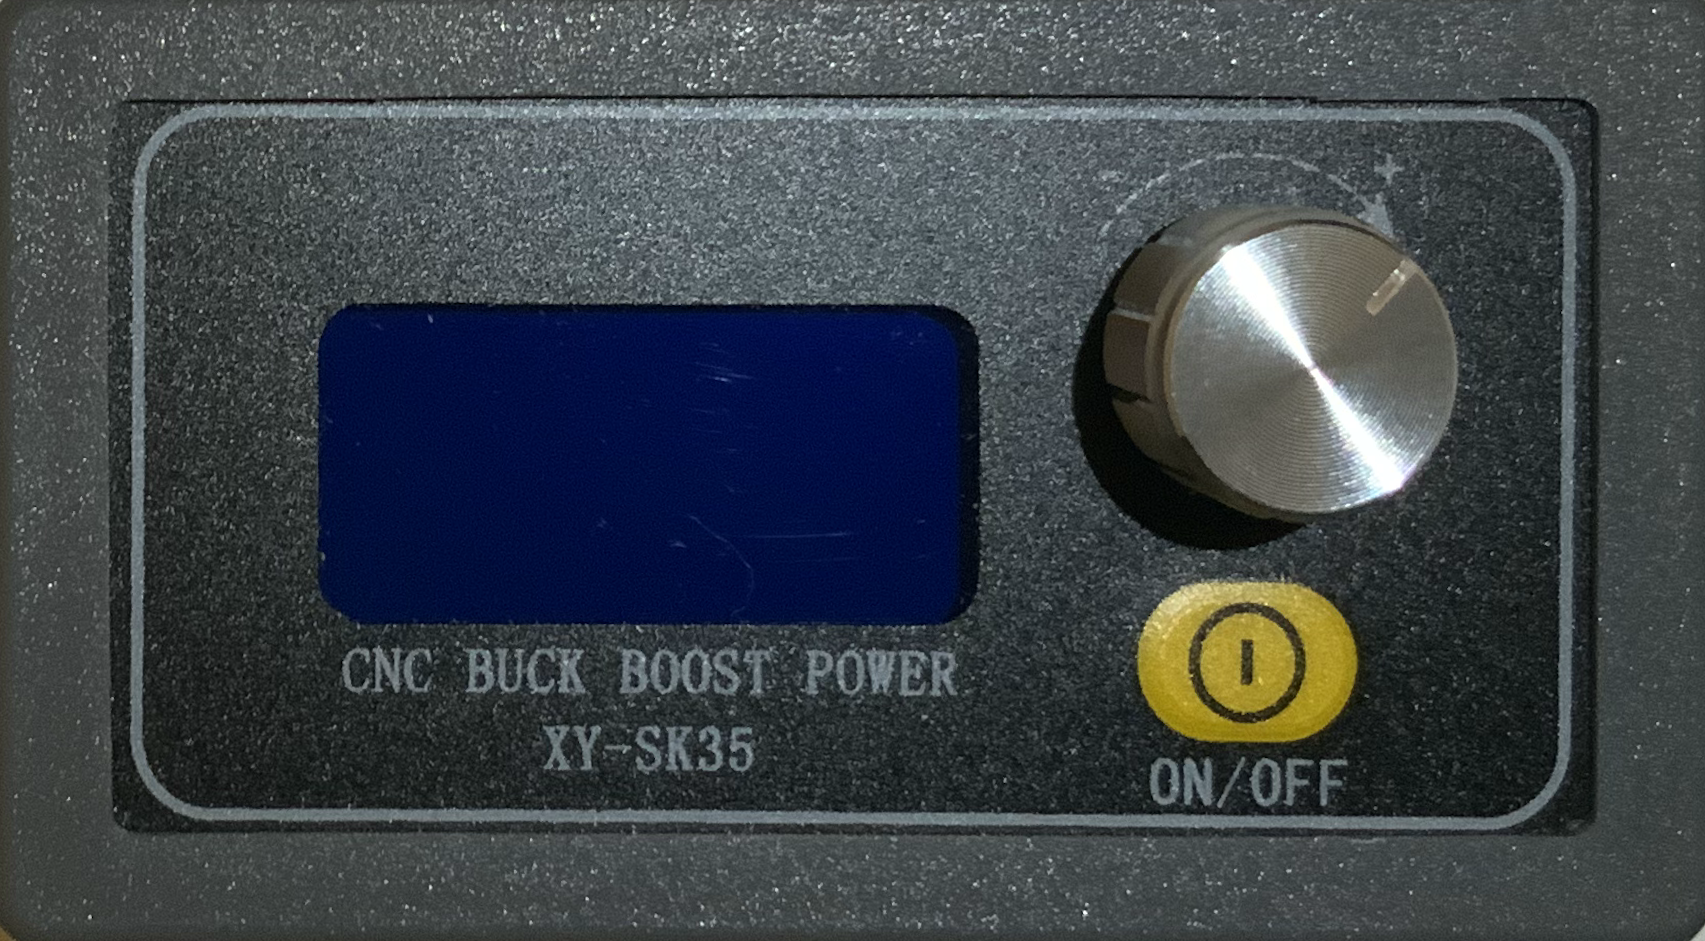
\includegraphics[width=0.4\textwidth]{figures/powerConverterModuleOff.png} & 
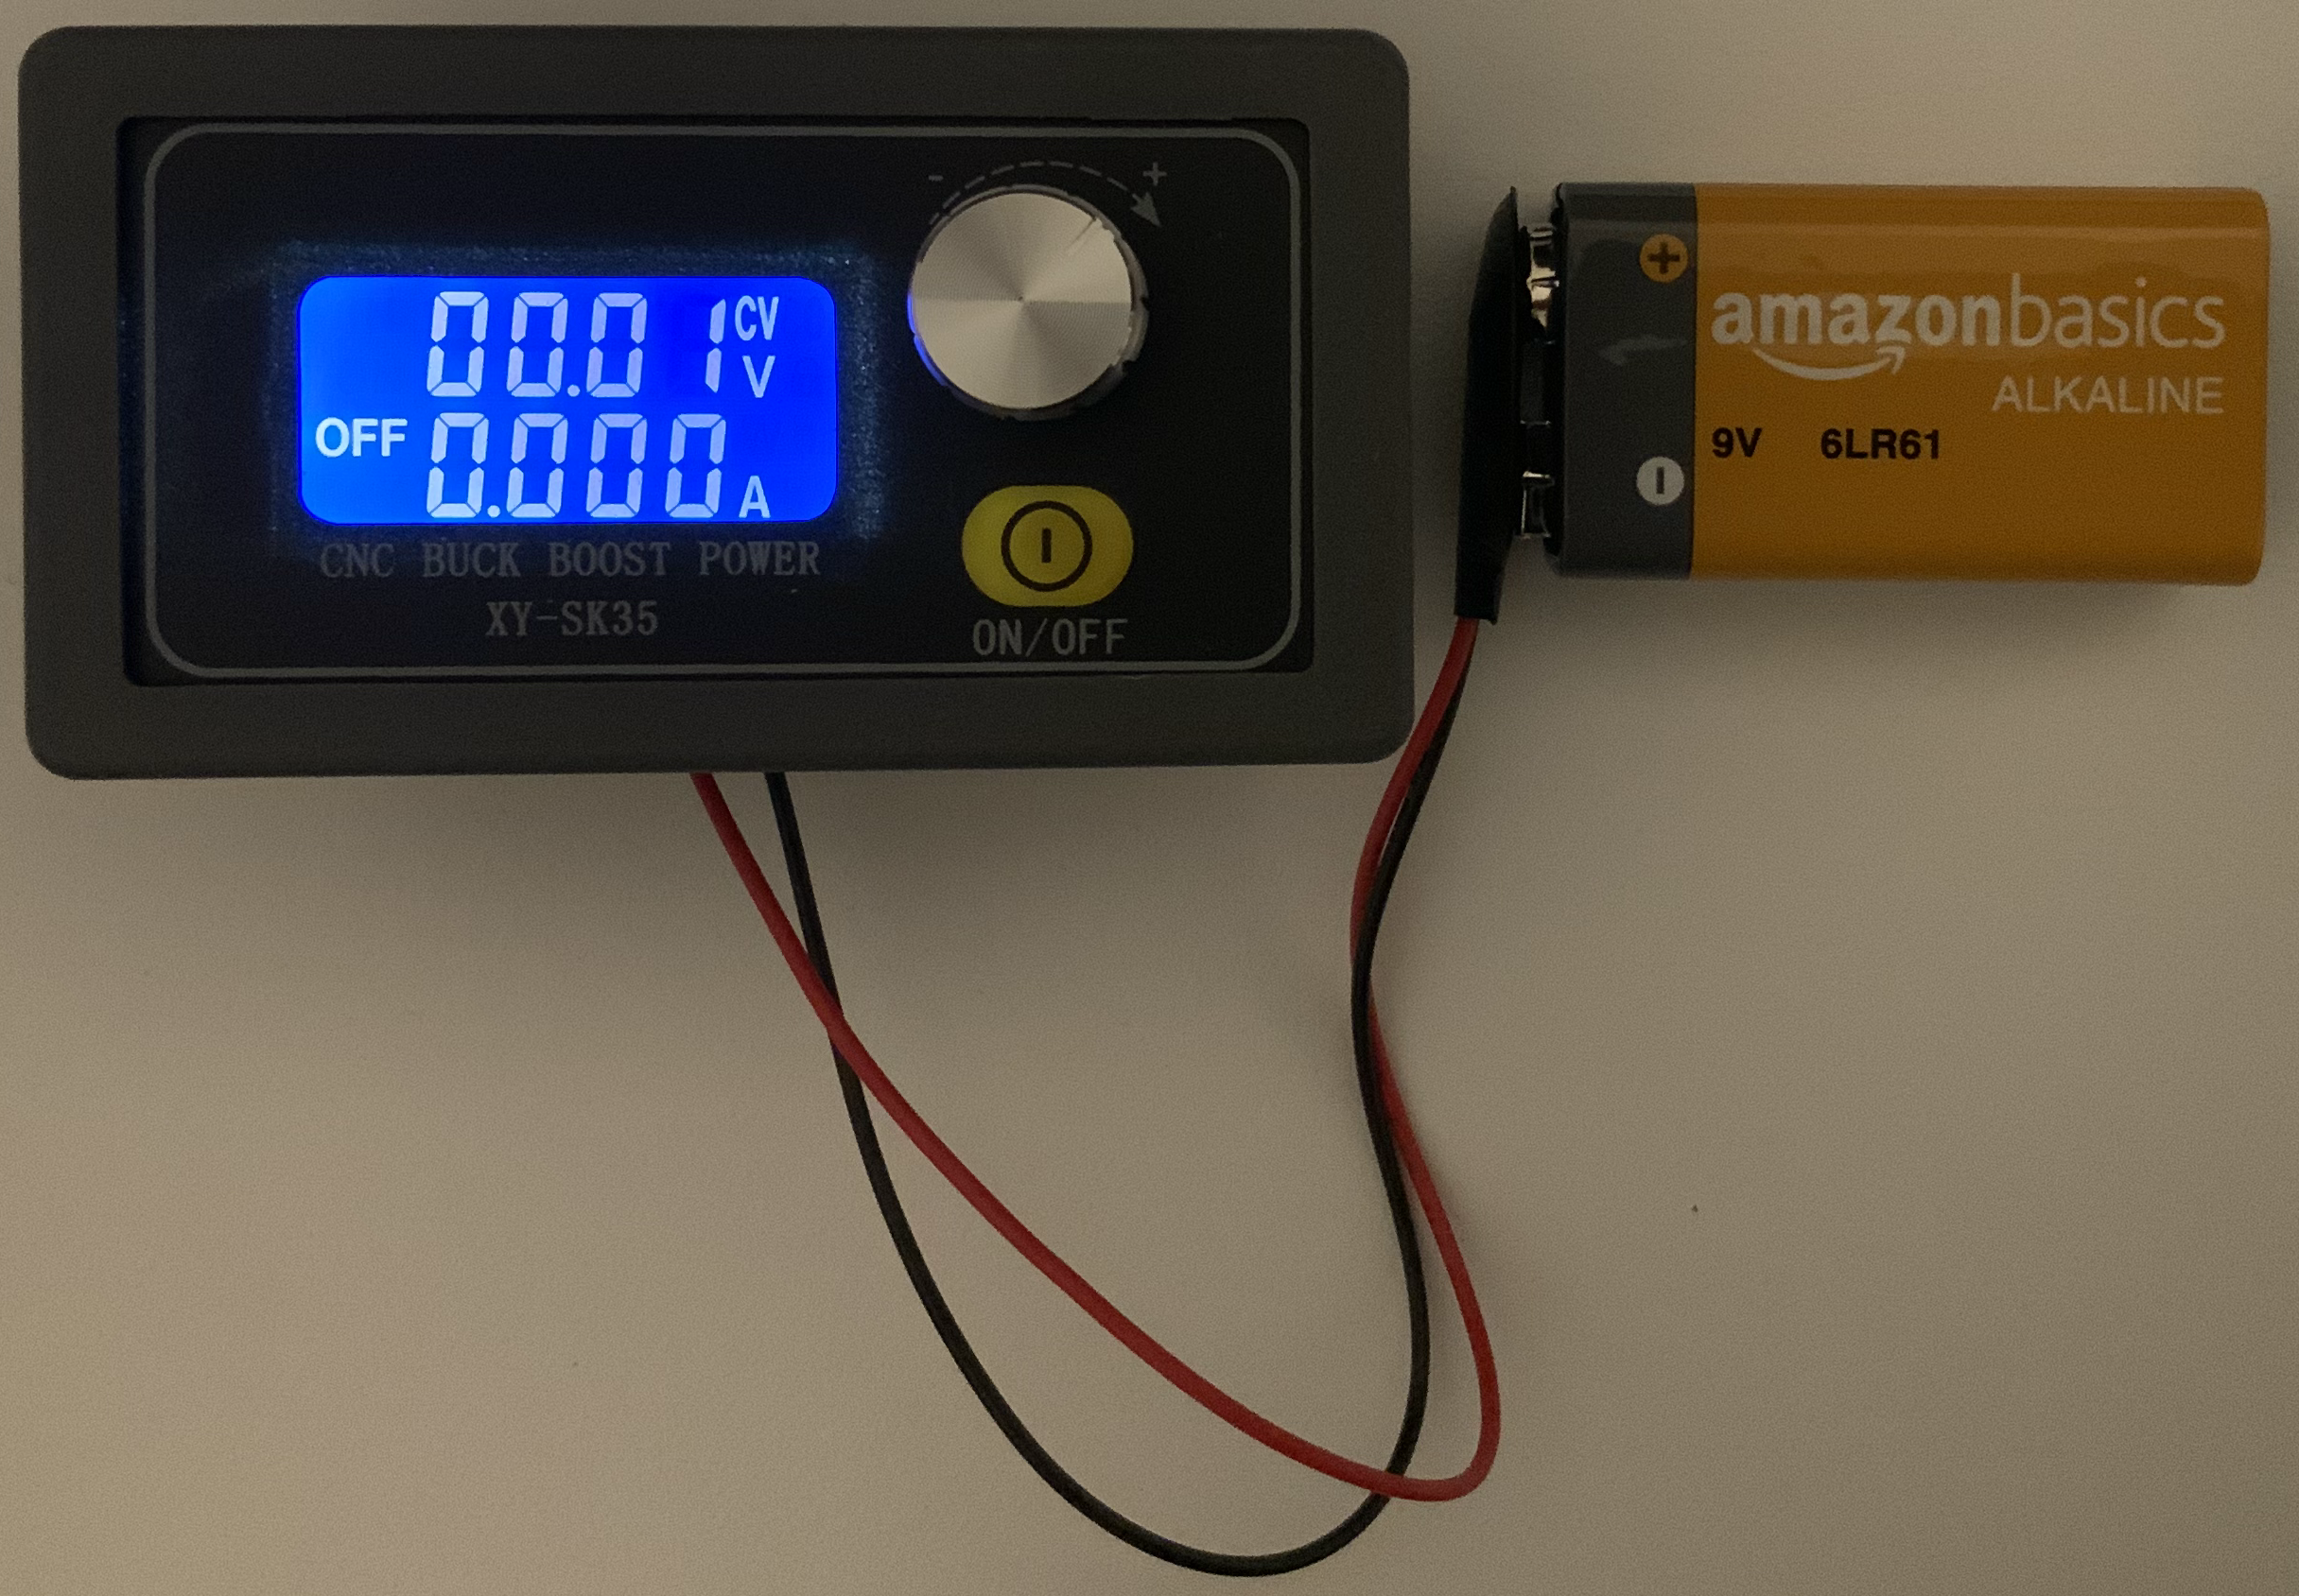
\includegraphics[width=0.4\textwidth]{figures/powerConverterModule.png}
\end{tabular}
\caption[UCTRONICS U6225 Power Supply Module]{Left: Power Supply Module off; Right: Power Supply Module with the positive terminal of the battery plugged in to $V_{IN+}$ and the negative terminal plugged in to $V_{IN-}$}
\label{fig:powerSupply}
\end{figure}

\subsection{Analog Devices M1K ADALM1000}
This instrument is shown in Figure \ref{fig:osc}. This instrument is the most versatile of all the instruments shown because it can perform multiple functions simultaneously. Not only can it act as an oscilloscope, it will also be our function generator for this semester.

\begin{figure}[ht!]
\begin{center}
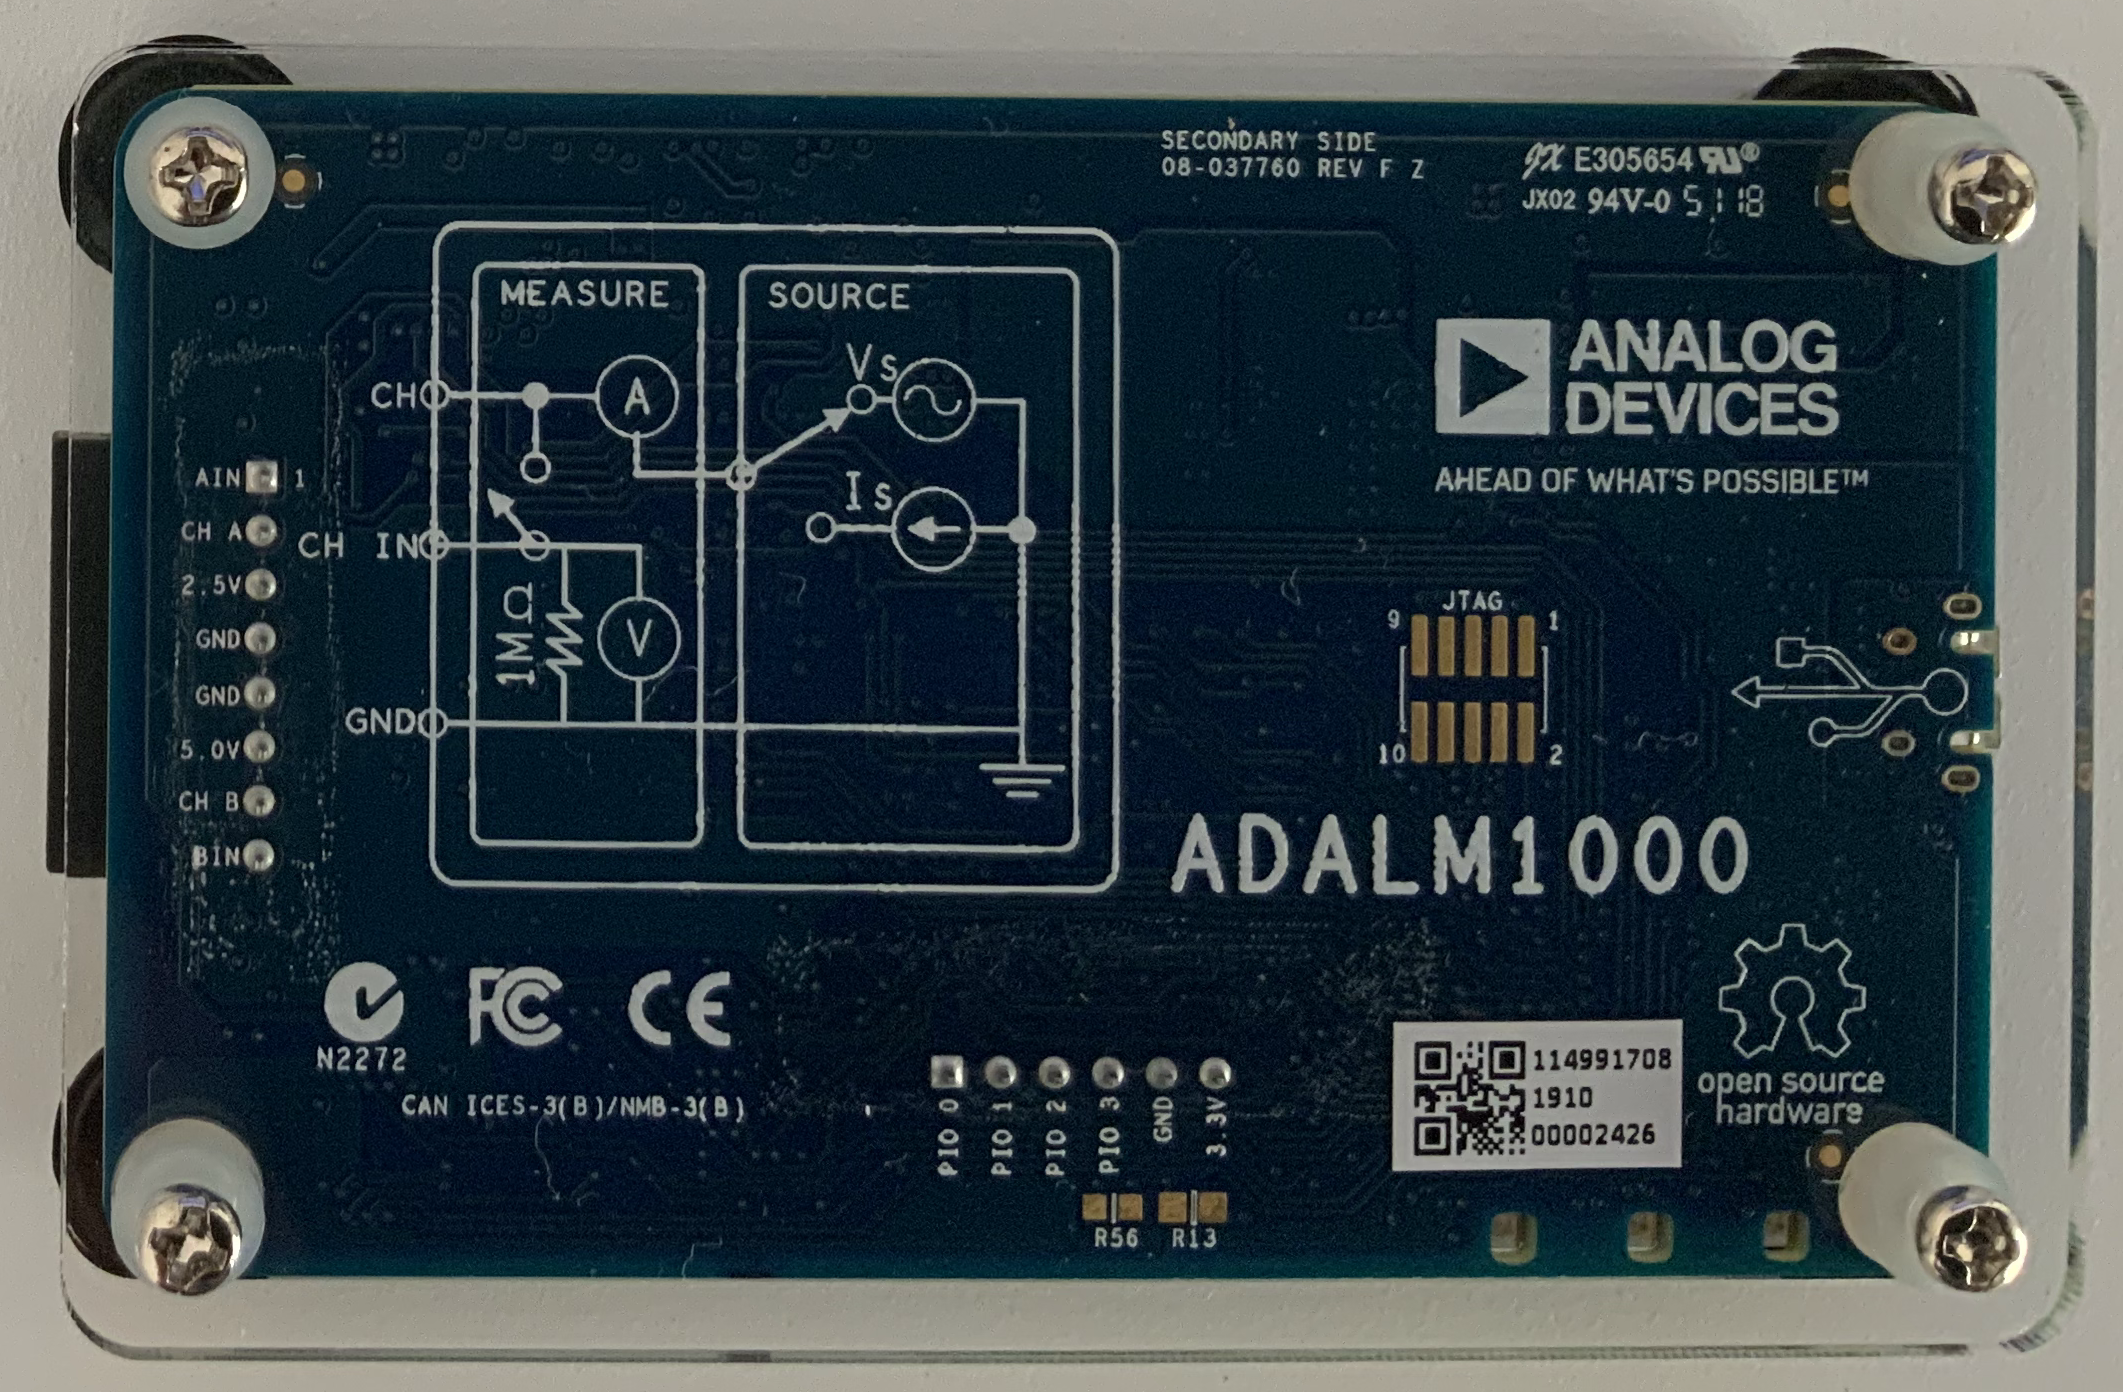
\includegraphics[width=0.5\textwidth]{figures/ADALM1000.png}
\caption[Analog Devices M1K ADALM1000]{Analog Devices M1K ADALM1000}
\label{fig:osc}
\end{center}
\end{figure}

You will be interacting with this instrument through a software called Pixelpulse2. Instructions on how to download Pixelpulse2 are included in Section 3.

\subsection{Jameco Breadboard}
You've probably seen this exact breadboard model in your previous ECE laboratories. You will be using this breadboard to build most of your circuits. Remember that any components placed in a row will be electrically connected to anything else placed in that row.

\begin{figure}[ht!]
\begin{center}
\includegraphics[width=0.4\textwidth, angle=90]{figures/breadboard.png}
\caption[Jameco Breadboard]{Jameco Breadboard}
\label{fig:breadboard}
\end{center}
\end{figure}

\subsection{AstroAI AM33D Multimeter}
This instrument is used to measure voltages, currents, and resistances. When configured to measure voltage, it is a voltmeter. When configured to measure current, it is an ammeter. When configured to measure resistance, it is an ohmmeter. Remember, you may have to change the terminal that the red lead is connected to in order to make certain measurements. 

\begin{figure}[ht!]
\begin{center}
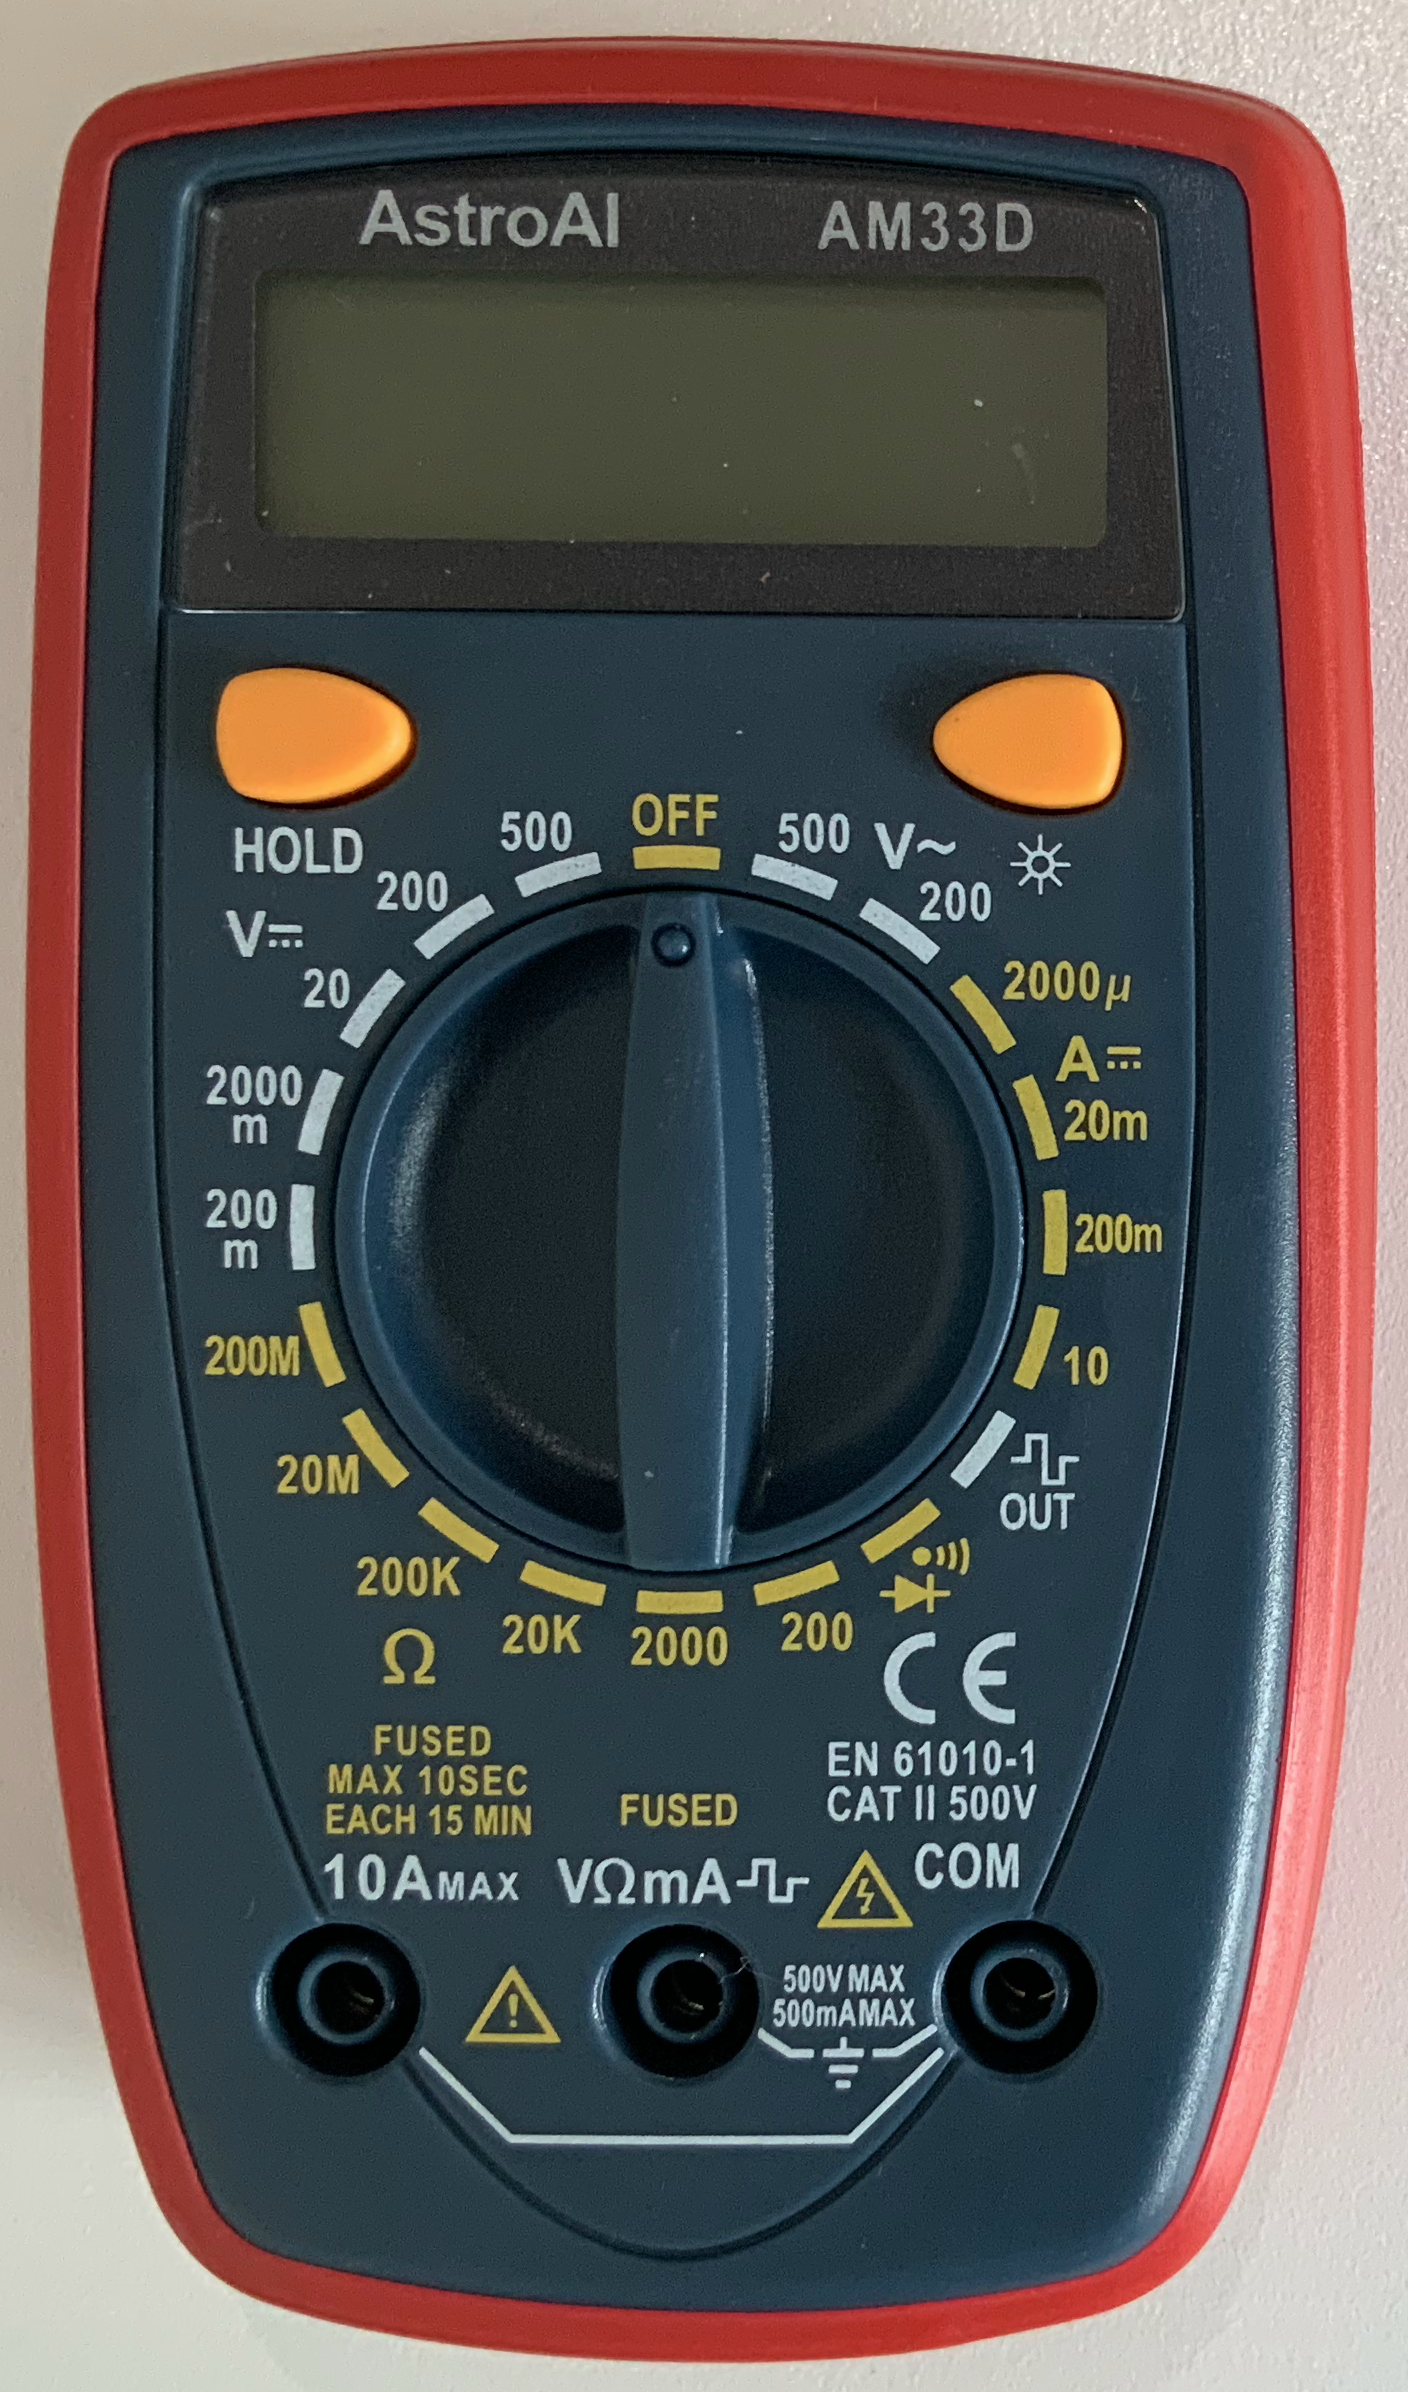
\includegraphics[width=0.4\textwidth]{figures/multimeter.png}
\caption[AstroAI AM33D Multimeter]{AstroAI AM33D Multimeter}
\label{fig:multimeter}
\end{center}
\end{figure}

\newpage
\section{Laboratory Preparation}
\subsection{Download and Install Pixelpulse2}
You can find the download link for Pixelpulse2 \href{https://github.com/analogdevicesinc/Pixelpulse2/releases/tag/v1.0.4}{here}. If you are on a Windows device, download {\tt Pixelpulse2\_win\_setup.exe}. If you are on a Mac, download {\tt Pixelpulse2-v1.0.4.dmg.zip}. After following the installation instructions, open Pixelpulse2. Confirm your application looks like the image below.

\begin{figure}[ht!]
\begin{center}
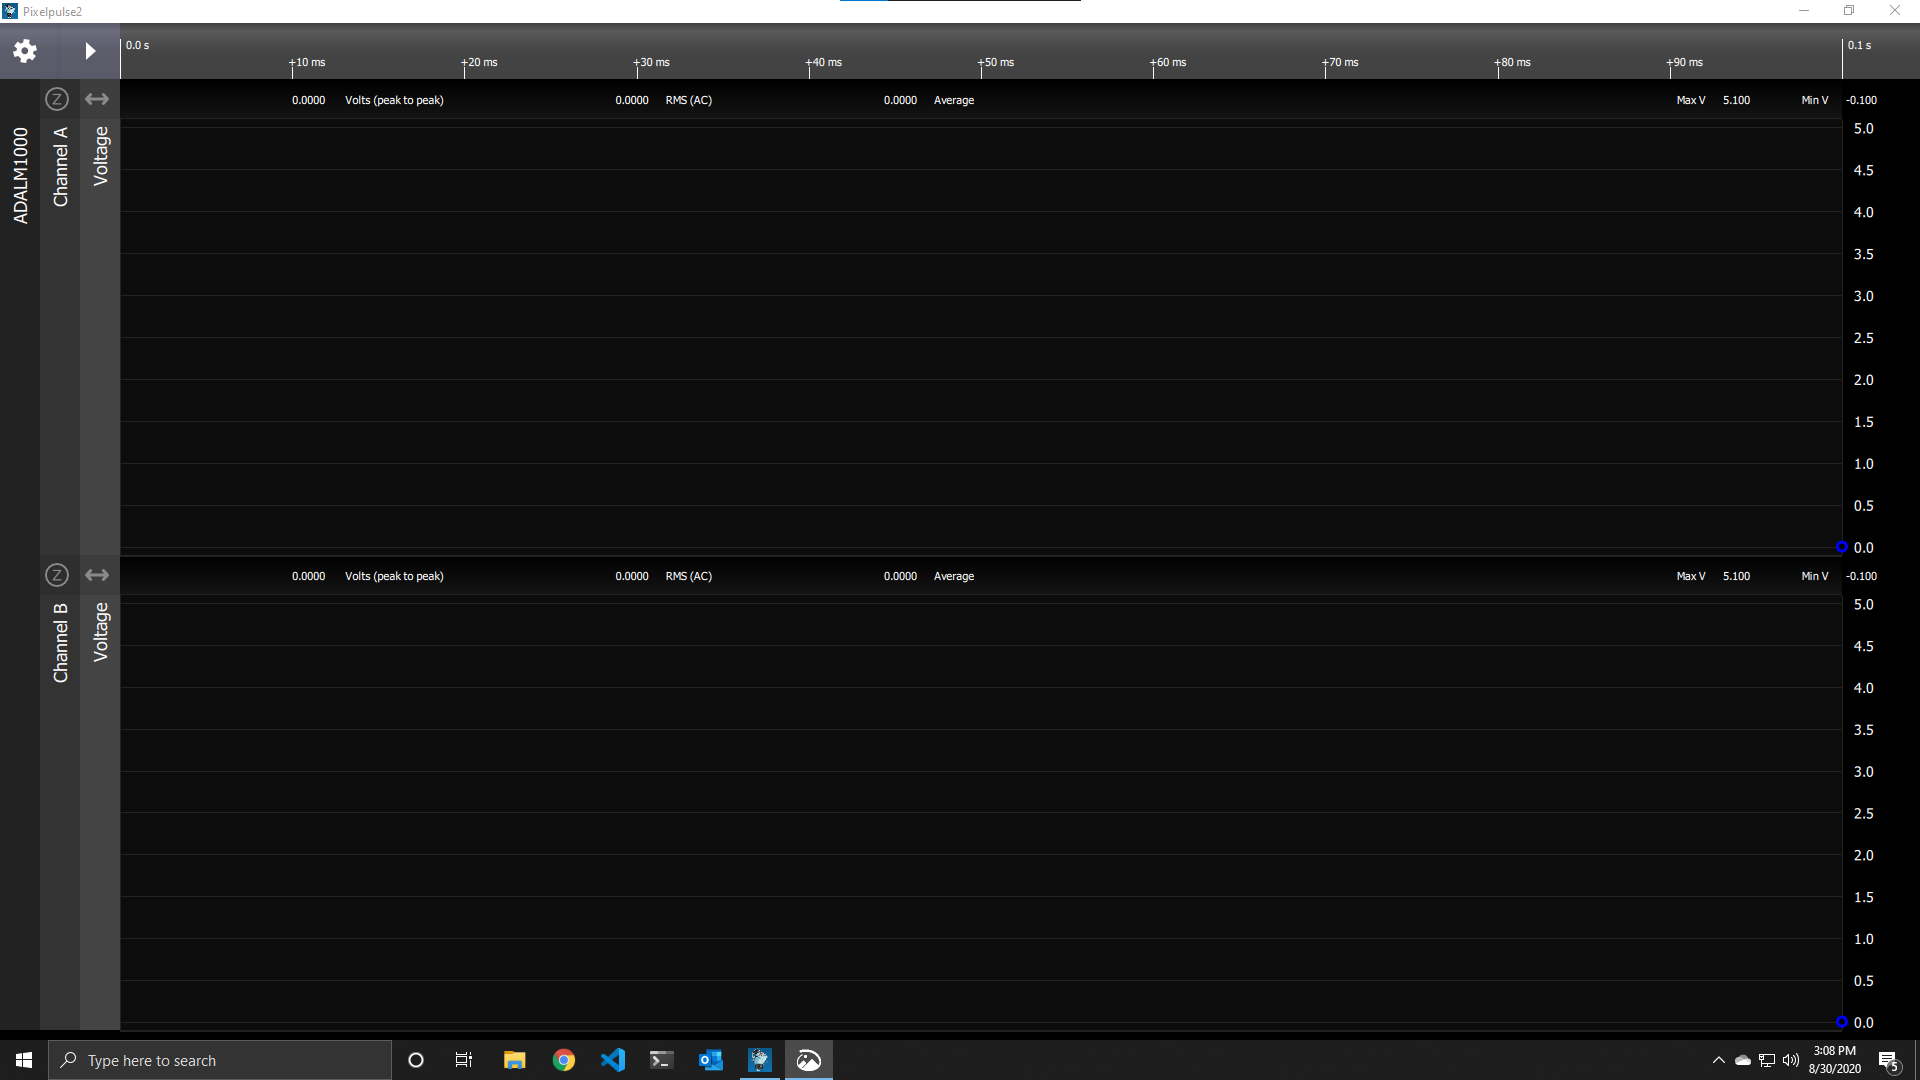
\includegraphics[width=0.9\textwidth]{figures/Pixelpulse2.png}
\caption[Pixelpulse2 GUI]{Pixelpulse2 GUI}
\label{fig:pixelpulse2}
\end{center}
\end{figure}

Note that you may have to update your device's firmware the first time you open the application. This should only take a few seconds. Unplug and plug the M1K back in once you receive a message saying that the firmware has been updated.

Also, you may want to check out \href{https://wiki.analog.com/university/tools/m1k/pixelpulse}{the wiki}.

\newpage
\section{Experimental Exercises}
\subsection{Practical Voltage and Current Measurements}
The standard resistor color code is shown on the wall in the laboratory above your lab bench. Most resistors have four colored bands. The first three bands indicate the nominal value of the resistor and the fourth band indicates the tolerance in its value. The first two bands form the mantissa and the third band represents the power of 10. A table of the resistance color code is included below for your convenience.

\def\arraystretch{1.4}
\begin{table}[ht!]
\caption{Resistance Color Code}
\centering
\begin{tabular}{|c|c|c|} \hline
Color 	& Mantissa Value & Multiplier \\ \hline \hline
Black 	& 0 & $10^0$ \\ \hline
Brown 	& 1 & $10^1$ \\ \hline
Red 	& 2 & $10^2$ \\ \hline
Orange 	& 3 & $10^3$ \\ \hline
Yellow	& 4 & $10^4$ \\ \hline
Green	& 5 & $10^5$ \\ \hline
Blue	& 6 & $10^6$ \\ \hline
Violet	& 7 & $10^7$ \\ \hline
Grey	& 8 & $10^8$ \\ \hline
White	& 9 & $10^9$ \\ \hline
\end{tabular}
\end{table}

The tolerance band is typically either Gold or Silver. A Gold tolerance band indicates that the measured value will be within 5\% of the nominal value. A Silver band indicates a 10\% tolerance. For example, a resistor with color code brown-black-red-silver indicates a nominal value of 1 k$\Omega$. The first two bands (Brown followed by Black) produce the mantissa of 10 and the third band (Red) is the exponent of two $(10^2 = 100)$. Therefore, the value of a brown-black-red-silver resistor is $10 \times 100 = 1$ k$\Omega$. Because the tolerance band is Silver, we can expect the measured value of the resistor to be between 900 and 1100 $\Omega$. 

\subsubsection{Ideal vs. Practical DC Voltmeters}
An ideal voltmeter has an infinite series resistance, i.e., it is practically an open circuit. Although it is impossible to make a physical voltmeter with infinite resistance, a well designed voltmeter exhibits a very large internal resistance. In some experiments, it is important to take into account the finite, non-ideal internal resistance of a DC voltmeter.

To determine the internal resistance of the voltmeter, set up a circuit as shown in Figure \ref{fig:voltcirc}.

\begin{figure}[ht!]
\begin{center}
\begin{circuitikz}[american, scale=1.5]
\ctikzset{resistors/scale=1.5, batteries/scale=1.5, instruments/scale=1.5}
\draw 
(0,0) to [resistor, l_=\SI{1}{M\ohm}, *-] ++(-3,0)
to [battery, l_=\SI{10}{V}] ++(0,-2)
to [short, -*] ++(3,0)
(0.25,-2) node[currarrow, rotate=180]{}
to [short] ++(0.75,0)
to [rmeter, t=V] ++(0,2)
to [short] ++(-0.75,0) node[currarrow, rotate=180]{}
;\end{circuitikz}
\caption[Circuit used to measure internal resistance of voltmeter]{Circuit used to measure the internal resistance $R_M$ of the voltmeter}
\label{fig:voltcirc}
\end{center}
\end{figure}

Note that you may need to use the 2.4 mm screwdriver to loosen and tighten the terminals of the power supply.

The voltmeter reads the voltage across itself, which includes its internal resistance. Because the circuit has only a single branch, the current flowing through the resistor also flows through the voltmeter. In this circuit, the source voltage $V_S = 10$ V and the DC voltage measured by the voltmeter is $V_M$. The current is given by the equation
\begin{align}
I = \frac{V_S - V_M}{R}.
\end{align}
From Ohm's Law, if we measure the current I and the voltage $V_M$, we can determine the resistance, $R_M$ of the voltmeter from 
\begin{align}
R_M = \frac{V_M}{I} = \frac{V_M}{\frac{V_S - V_M}{R}} = \frac{V_M}{V_S - V_M}R
\end{align}
To determine the internal resistance of the voltmeter, carry out the following steps:
\begin{enumerate}
\item Select a 1 M$\Omega$ resistor. 
\item Measure its resistance using the multimeter. 
\item Set the power supply to provide 10 V. Always remember to measure the voltage provided by the power supply either with the voltmeter or the scope. Do not rely on the digital display on the front panel of the power supply. 
\item Assemble the circuit in Figure \ref{fig:voltcirc}. 
\item Record the voltage $V_M$ measured by the voltmeter. 
\item Compute the internal resistance $R_M$ of the voltmeter (above) 
\end{enumerate}

\subsubsection{Ideal vs. Practical DC Ammeters}
An ideal ammeter has zero internal resistance so that the circuit in which it has been placed is not disturbed. An ideal ammeter is a short circuit. As with the voltmeter, however, no ammeter is ideal. Thus, all ammeters have some optimally small internal resistance.

To determine the resistance of the DC ammeter, set up a circuit as shown in Figure \ref{fig:ampcirc}.

\begin{figure}[ht!]
\begin{center}
\begin{circuitikz}[scale=1.5]
\ctikzset{resistors/scale=1.5, batteries/scale=1.5, instruments/scale=1.5}
\draw 
(0,0) to [resistor, l_=\SI{100}{\ohm}] ++(-4,0)
to [battery, l_=\SI{1}{V}] ++(0,-2)
to ++(4,0) 
to [rmeter, t=A] ++(0,2)
;\end{circuitikz}
\caption[Circuit used to measure internal resistance of ammeter]{Circuit used to measure the internal resistance $R_M$ of the ammeter}
\label{fig:ampcirc}
\end{center}
\end{figure}

According to Ohm's Law, the current in this circuit is given by
\begin{align}
I = \frac{V_S}{R + R_M}
\end{align}
By measuring the current $I$ and the source voltage $V_S$, and knowing the value of the series resistance $R$, we can determine the ammeter resistance $R_M$ from
\begin{align}
R_M = \frac{V_S}{I} - R \label{eq:amres}
\end{align}
In the procedure that follows, it is extremely important that you take precise and accurate measurements. Record each measurement as precisely as the instrument will allow.
\begin{enumerate}
\item Select a 100 $\Omega$ resistor. Measure and record its resistance. 
\item Set the voltage of the DC Voltage Source to 1 V.
\item Assemble the circuit shown in Figure \ref{fig:ampcirc}. Set the multimeter to the ammeter mode for DC current measurement.
\item Use the oscilloscope to measure the voltage $V_S$ across the DC power supply (use the ``average'' measurement).
\item Measure the DC current $I$ using the ammeter. 
\item Determine the value of $R_M$ from Equation \eqref{eq:amres}. 
\end{enumerate}

\subsection{Measurements of Time-Dependent Sources}
In this section, we will be using the M1K as a function generator to provide a time-dependent voltage waveform which will then be measured using the other channel of the M1K. \textbf{It is important NOT to let the leads of the M1K touch each other.} If the function generator leads touch each other, either the internal fuse will blow or serious damage to the instrument will occur. It is very important that you keep this in mind at all times. If the internal fuse blows, the device will need to be replaced.

The function generator has an internal resistance of 50 $\Omega$. The voltage displayed on its front panel is the voltage that would appear at its terminals if it were connected to a 50 $\Omega$ load. Under open-circuit conditions, the voltage across the terminals of the function generator is twice as large as the value indicated on the Pixelpulse2 software. \textbf{This important concept is often misunderstood.}

\subsubsection{Periodic Pulsed Waveform}
Asynchronous reset pulses produced by integrated circuit (IC) chips can often be difficult to detect.  These pulses are important, however, and are often used in circuits to trigger a subsequent event, such as a clock ticking or a ``clear'' command to be sent.  The 74HC85 comparator chip is a high-speed Si-gate CMOS (Complementary Metal-Oxide-Semiconductor) device, for example, that produces a fast 250 ns pulse with a 25 ns rise and fall time, respectively.   Such a pulse is very quick and thus hard to detect on the oscilloscope without proper triggering.  In this exercise, you will simulate a pulse similar to the one produced by the 74HC85 chip and learn to trigger and analyze the resultant waveform.

\begin{enumerate}
\item Set the function generator to produce a pulsed waveform by pressing the \fbox{Pulse} button on the front panel
\item Set the pulse parameters to produce the following: 
\begin{itemize}
\item 250 ns width
\item 10 Hz
\item 5 V amplitude
\item 25 ns edges waveform
\end{itemize}
\item Connect the oscilloscope channel-1 probe directly to the leads on the function generator and turn on the output of the function generator.
\item Under the Trigger menu on the oscilloscope, turn on \fbox{Edge} mode, and adjust the \fbox{Level} knob. It might also be helpful to set the trigger mode to \fbox{Normal} . 
\item Determine the width of the waveform and its edges. Does it agree with what you expected based on the input pulse parameters? Why or why not? Explain.
\item \textbf{Capture the resultant waveform on the oscilloscope screen} and save it to document your laboratory experiments.
\end{enumerate}

Before you leave, please be sure to \textbf{clean up} the lab station where you worked, putting away all components, wires, probes, and cables as you found them. Also remember to turn off all the equipment you used. There are lab sections that follow you. Please be courteous in your practices.

\newpage
\section{Questions}
\begin{enumerate}
\item Define and differentiate between precision, accuracy, and resolution in electrical measurements. What is the ``resolution'' of a digital display? Compare the resolution of the digital display on the front panel of the DC power supply to the display on the front panel of the multimeter. Why must you use the multimeter to set the DC supply to 0.75 V? (The Agilent product manual available online for these instruments may be useful in answering this question.)
\item Suppose you want to produce a sinusoidal waveform with 5 V peak-to-peak voltage across a 25 $\Omega$ load with the function generator. When you do so, what will be the peak-to-peak voltage actually displayed on the front panel of the function generator and why? (Assume that the function generator has a standard internal 50 $\Omega$ resistance.)
\item Look up the internal resistances for both the voltmeter and ammeter capabilities for the Agilent 34410A Digital Multimeter used in lab. How do these values compare to the internal resistances you measured in section 3.1? Give percent errors.
\item In section 3.3, you compensated the oscilloscope probe on the Agilent DSOX1102G oscilloscope at your laboratory bench.  Making the assumption that the 10x scope probe has a 9 M$\Omega$ series impedance (i.e. you can ignore any small probe tip capacitance), determine the maximum value of $C_{\mathrm{comp}}$ from your measurement of $\tau$, the time constant.  Report two $C_{\mathrm{comp}}$ values---one determined when the oscilloscope probe was fully under-compensated and one when the oscilloscope probe was full over-compensated.  Include in your assignment the oscilloscope waveforms you used to determine $\tau$. 
\end{enumerate}
Submit the answers to these questions along with an extension and all of the other below-listed items in the rubric in your Lab 1 write-up in order to receive all possible points. 

\textit{Laboratory Notebooks:  There is no laboratory notebook requirement in ECE 230L, however, the use of a notebook for recording work performed in the laboratory is a very good practice and one that is encouraged.  Tips and pointers on how to maintain an excellent laboratory notebook are available on the lab site or can be obtained by speaking with your TA or instructor. It is a great idea to add comments and notes to your notebook before leaving lab---this is best done while the work is fresh in your mind!}
\newpage
\section{Extension}
To earn up to an additional 7 points (bringing the total possible points up to 100), you must show evidence of independent thought. This may include (but is not limited to):
\begin{itemize}
\item The oscilloscopes provided in the ECE 230L laboratory are high quality, expensive, state of the art devices.  However, there are even more expensive ‘scopes available.  What parameters make for a better oscilloscope and why?  Consider in particular sampling rate, speed, MHz, …
\item When would a compensated probe be necessary when measuring time-varying waveforms?  Give extreme cases and explain how an undercompensated and overcompensated probe would adversely affect the measurement.
\item Explain in circuit-level detail the functioning of the 10x, \SI{100}{\mega\ohm}, compensated oscilloscope probe.  Be sure to show measured signal, signal output, and the effect of the \SI{100}{\mega\ohm}.  Mention the internal capacitor and why compensation is necessary.
\item Explore in depth another question that piqued your interest as you completed this laboratory.
\end{itemize}
The number of additional points awarded depends on the quality and extent of your independent contribution.

\newpage
\begin{appendices}
\section{Oscilloscope Probe Calibration And Related Exercises}
\subsection{Oscilloscope Probe Calibration}
Probe compensation is the process of adjusting the $RC$ divider so the probe maintains its attenuation ratio over the probe's rated bandwidth. Make sure you check the probe compensation when you first connect a probe to an oscilloscope input because it may have been adjusted previously to match a different input.   

The Agilent DSOX1102G oscilloscope has a square wave reference signal available on the front panel to use for compensating the probe.

In the procedure that follows, we calibrate the probe.
\begin{enumerate}
\item Attach the probe tips to the probe compensation terminal and connect the probe to an input of the scope. Check to make sure the probe is at 10x magnification.
\item View the square wave reference signal on the screen and make adjustments on the probe capacitance using a small screw driver so that the square waves on the scope screen look square.
\item Probe compensation is now complete!
\end{enumerate}

\begin{figure}[ht!]
\begin{center}
\centering
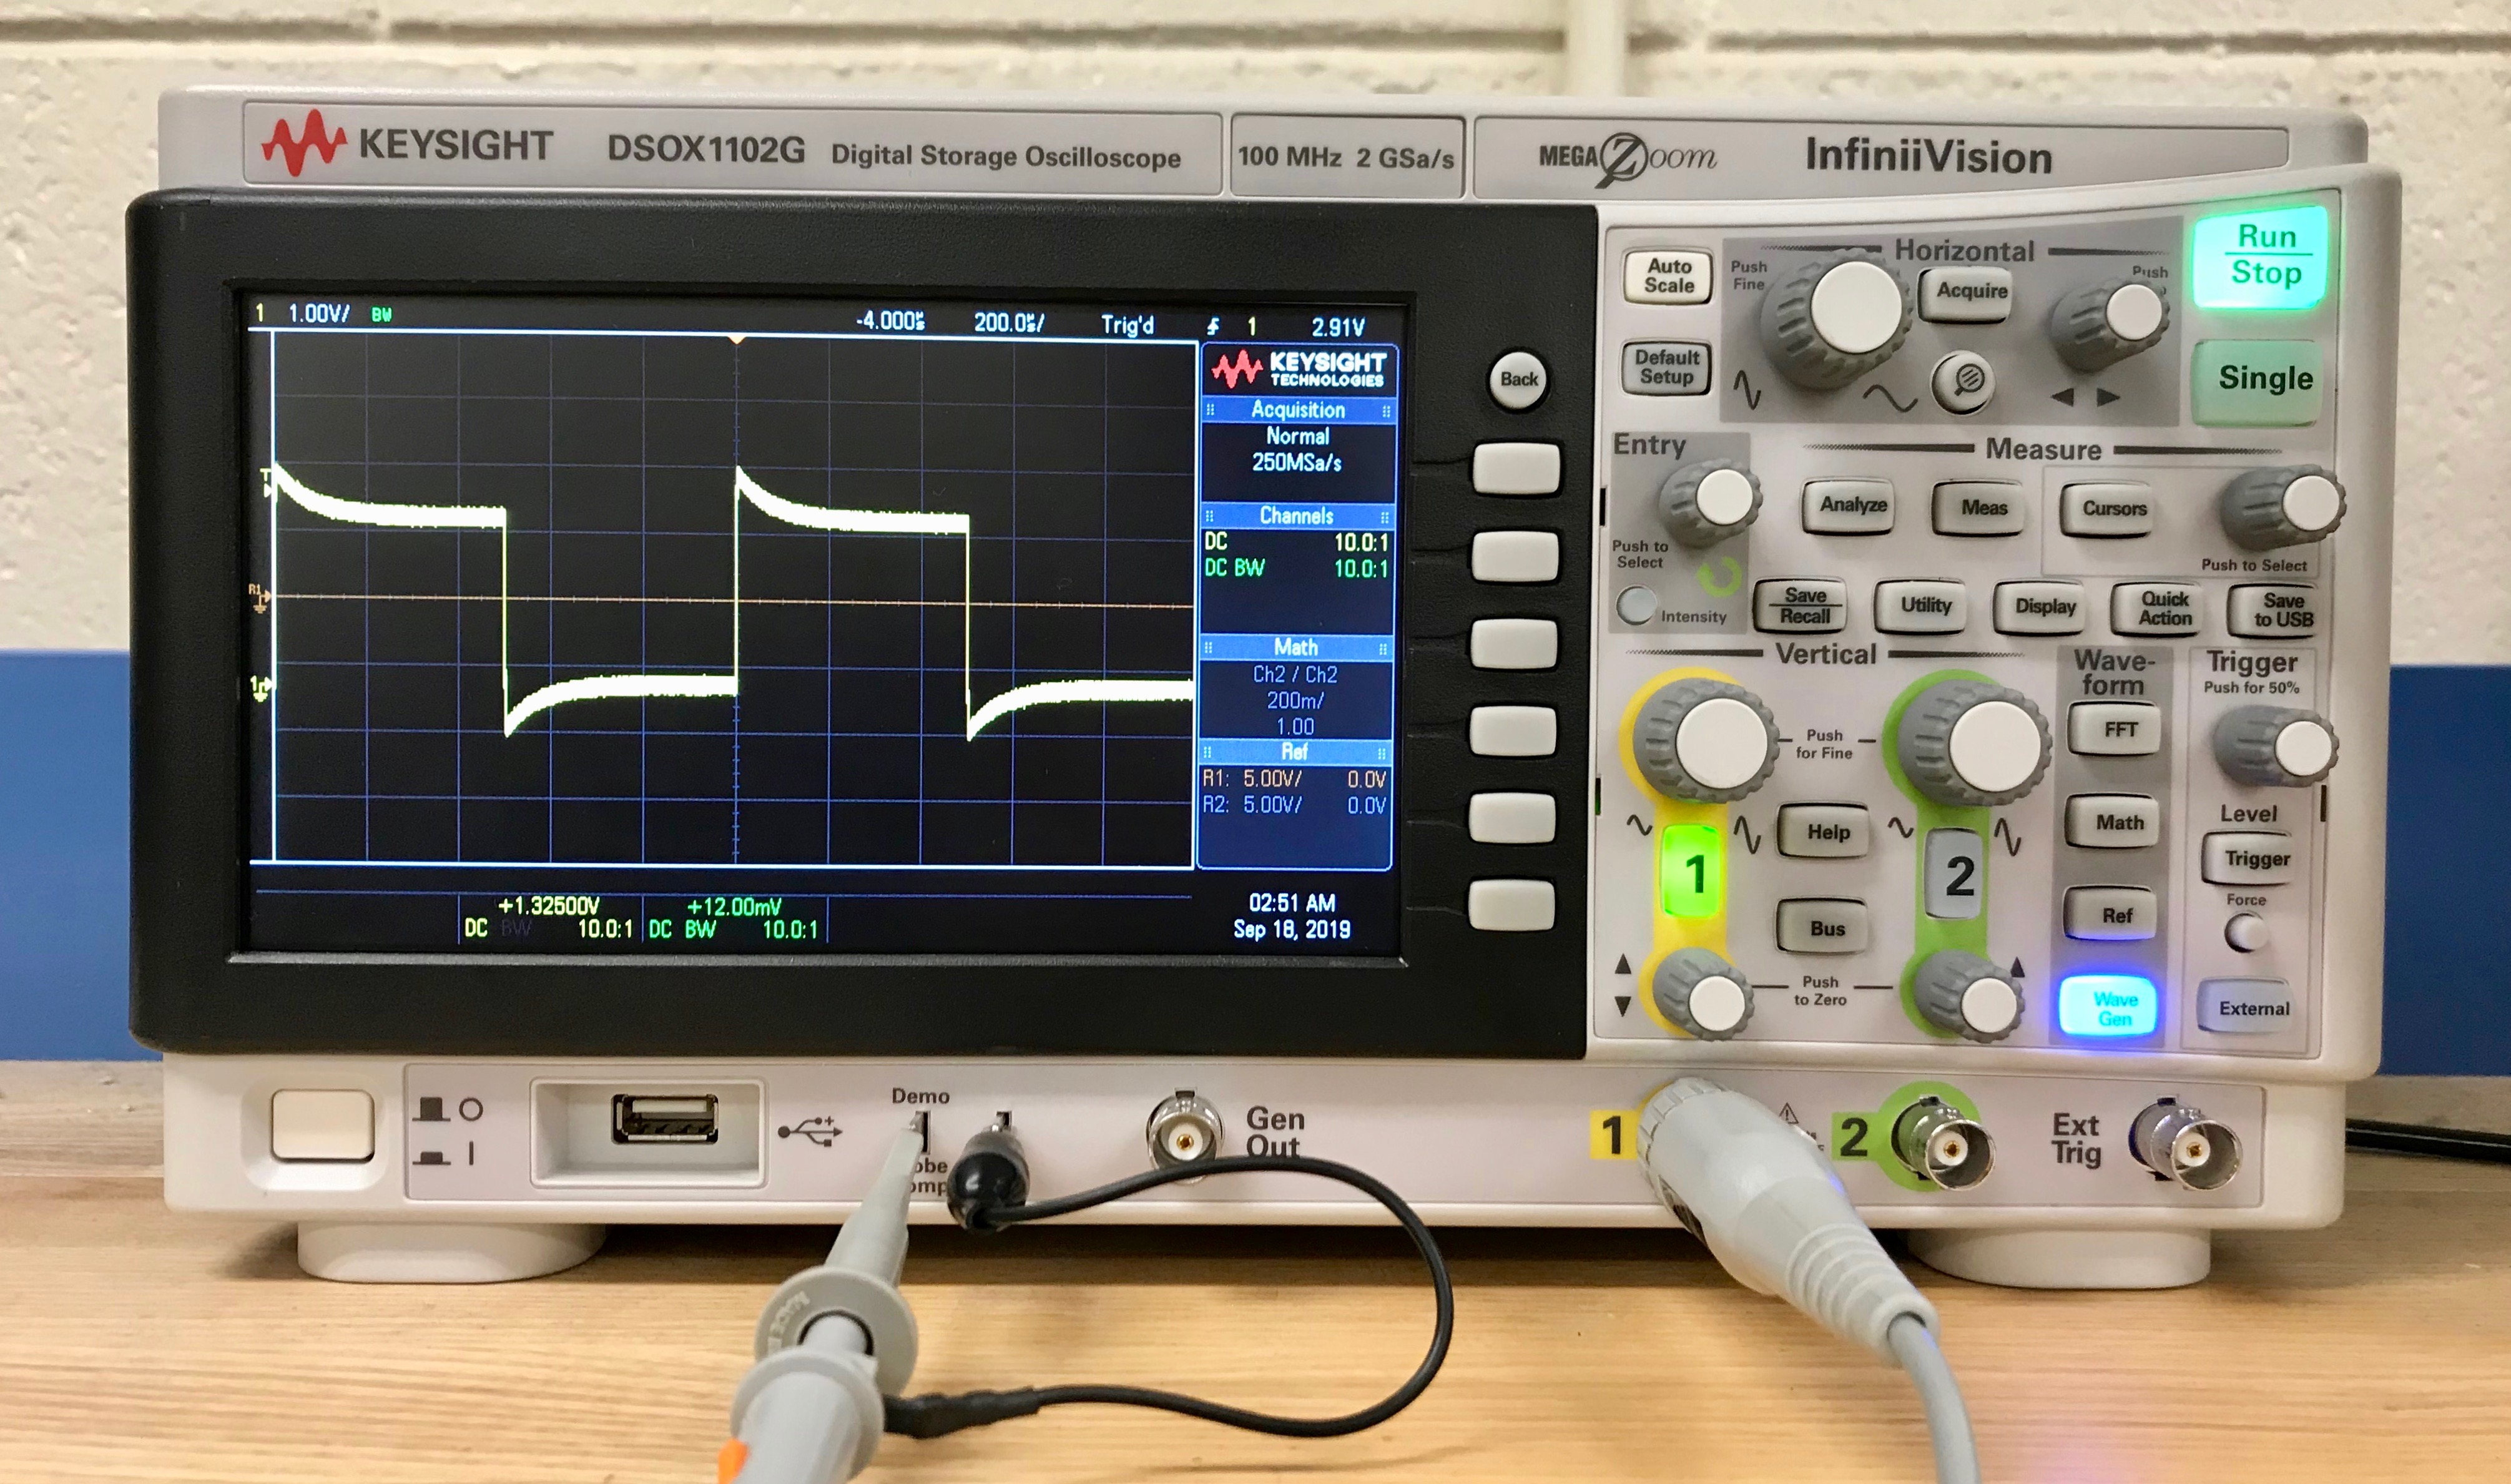
\includegraphics[width=0.9\textwidth]{figures/OscProbeComp.jpeg}
\caption[Oscilloscope Probe Calibration]{The probe tip attaches to the metal terminal labeled ``Probe Comp''}
\label{fig:oscprobecomp}
\end{center}
\end{figure}

Now, you will full under-compensate and over-compensate the oscilloscope probe to determine the approximate value of the variable compensation capacitor $(C_{\mathrm{comp}})$ which is part of the oscilloscope's 10x probe.

\begin{itemize}
\item[4.] Measure two instances of the time constant, $\tau$---one when the oscilloscope probe is fully under-compensated and one when the oscilloscope probe is full over-compensated. The oscilloscope waveforms should appear similar to those shown in Figure \ref{fig:oscdifcomp}.
\end{itemize}

To solve for $\tau = RC$, we use the equation 
\begin{align}
\Delta V_C = \Delta V_{\mathrm{max}} \cdot e^{-t / RC}.
\end{align} 
However, we must first find $\Delta V_{\mathrm{max}}$. This is the difference between the maximum voltage $V_{\mathrm{max}}$ on the left side of the wave and the stable voltage $V_{\mathrm{stable}}$ on the right side of the wave. This value should be positive for under-compensated probes and negative for over-compensated probes (and 0 for well-compensated probes). Next, we find $\Delta V_C$ for an under-compensated probe by using 
\begin{align}
\Delta V_C &= \Delta V_{\mathrm{max}} \cdot e^{-t / \tau}. \label{eq:tau} \\
\intertext{Now, we set t = $\tau$}
\Delta V_C &= \Delta V_{\mathrm{max}} \cdot e^{-\tau / \tau} \\
\Delta V_C &= \Delta V_{\mathrm{max}} \cdot e^{-1}
\intertext{Since $\Delta V_{\mathrm{max}}$ and $e^{-1}$ are known values, we have solved for $\Delta V_C$. Note that for an over-compensated probe, we replace (\ref{eq:tau}) with}
\Delta V_C &= \Delta V_{\mathrm{max}} \cdot [1 - e^{-t / \tau}].
\end{align}

Now, we can measure $\tau$ for both an under- and over-compensated scope. We do so by first adding $V_{\mathrm{stable}} + \Delta V_C$ to get the value of the voltage at one time constant. We'll call this value $V_{\tau = 1}$. Finally, we use the oscilloscope's \fbox{Cursor} to measure the time $\tau$ it takes for the wave and $V_{\tau = 1}$ to intersect.

\begin{figure}[ht!]
\begin{center}
\begin{tabular}{ccc}
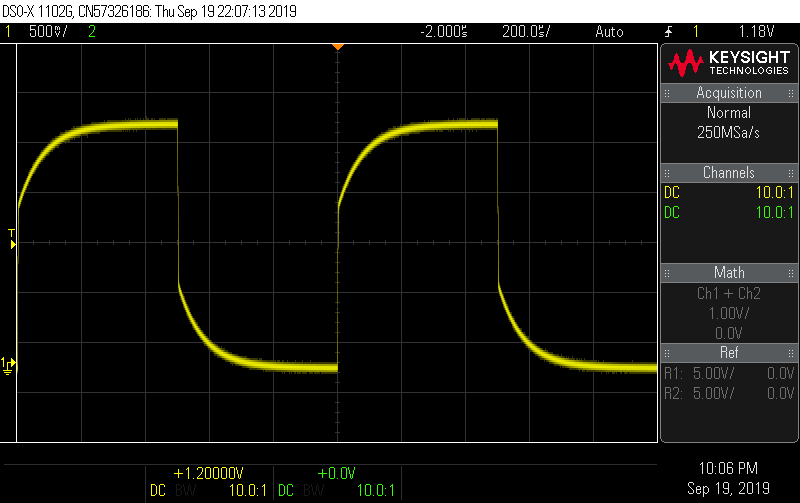
\includegraphics[width=0.31\textwidth]{figures/overcomp.png} & 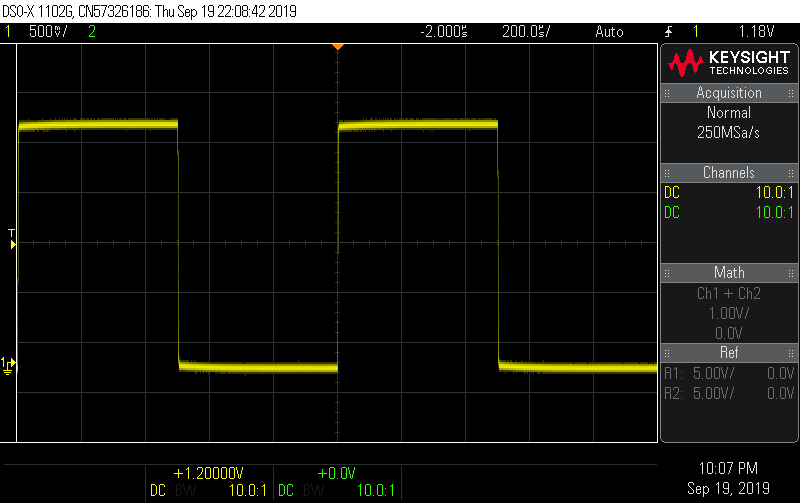
\includegraphics[width=0.31\textwidth]{figures/wellcomp.png} & 
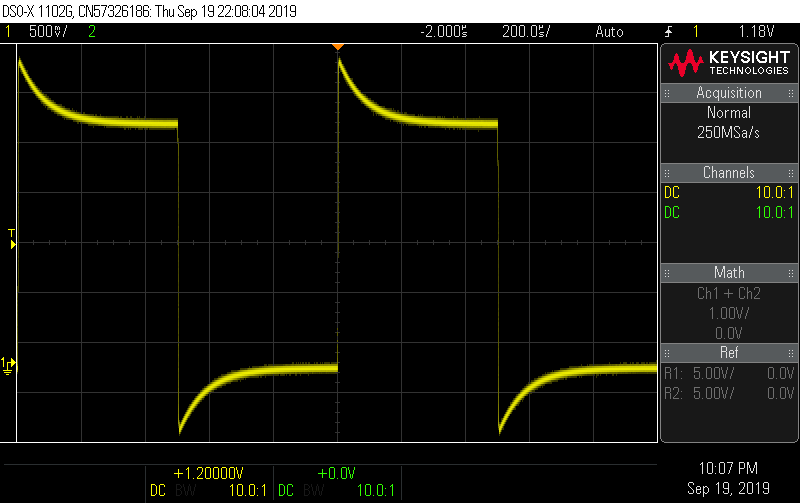
\includegraphics[width=0.31\textwidth]{figures/undercomp.png}
\end{tabular}
\end{center}
\caption[Square waves from probes with different compensations]{Square waves from probes with different compensations. From left to right: over-compensated, well-compensated, under-compensated.}
\label{fig:oscdifcomp}
\end{figure}

As you can see in Figure \ref{fig:oscdifcomp}, when compensating the probe using the oscilloscope's reference signal, you can have either overshoot or undershoot on the square wave. You can attach the probe tip to the probe compensation terminal and connect the probe to an input of the scope. Viewing the square wave reference signal, make the proper adjustments on the probe using a small screw driver so that the square waves on the scope screen look square. What you are adjusting is a variable capacitor at the tip of the probe. If low-frequency adjustment is not properly made, this will result in high-frequency inaccuracies in your measurements.  It's very important to make sure this compensation capacitor is correctly adjusted.
\end{appendices}


%____________________________________________________________________________
%
%	Grading Rubric
%____________________________________________________________________________
\newpage
\phantomsection
\addcontentsline{toc}{section}{Grading Rubric}
\markboth{Grading Rubric}{Grading Rubric}
\hspace{0pt}
\vfill
\begin{table}[ht!]
\caption{ECE 230L Laboratory 1 Grading Rubric}
\centering
\begin{tabular}{l|c} \hline
Criteria & Points Possible \\ \hline \hline
\textbf{Internal Resistance of a Voltmeter}					& \textbf{12} \\
Circuit Diagram												& 4 \\
Actual measurements for $V_M, V_S$, and $R$					& 4 \\
Equation and $R_M$ value									& 4 \\ \hline
\textbf{Ideal vs. Practical DC Ammeter}						& \textbf{12} \\
Circuit Diagram												& 4 \\
Actual measurements for $V_M, V_S,$ and $R$					& 4 \\
Equation and $R_M$ value									& 4 \\ \hline
\textbf{Measurements of Time-Dependent Sources}				& \textbf{6} \\
Observed width of the waveform and its edges				& 3 \\
Image of waveform 											& 3 \\ \hline
\textbf{Question 1}											& \textbf{12} \\ \hline
\textbf{Question 2}											& \textbf{12} \\ \hline
\textbf{Question 3}											& \textbf{12} \\ \hline
\textbf{Question 4}											& \textbf{12} \\ \hline
\textbf{Extension}											& \textbf{7} \\ \hline
\textbf{Total}												& \textbf{100} \\ \hline
\end{tabular}
\end{table}
\vfill
\hspace{0pt}
%____________________________________________________________________________
%
%	End{PROBLEMS}
%____________________________________________________________________________
\end{document}
